\documentclass{article}
\usepackage[margin=2.5cm, top=2.5cm, headheight=25pt]{geometry}
\usepackage{amsmath, amssymb, enumitem, fancyhdr, graphicx}
\usepackage[indent=20pt]{parskip}
\usepackage[hidelinks]{hyperref}
\usepackage{xcolor}
\usepackage{listings}
\usepackage{subcaption}
\usepackage{url}
\usepackage[most]{tcolorbox}
\usepackage{lastpage}
\usepackage{tikz}
\usepackage{circuitikz}

\usetikzlibrary{arrows, positioning}
\tcbuselibrary{listingsutf8} % Support for lstlistings within tcolorbox

\newtcolorbox[auto counter, number within=section]{question}[1][]{%
    colframe=gray!80,                      % Dark gray frame
    colback=gray!5,                       % Light gray background
    coltitle=black,                        % Black title
    title=\textbf{Question~\thetcbcounter}, % Bold title
    fonttitle=\bfseries\large,             % Subtle title font size
    rounded corners,                   % Slightly more rounded corners
    boxrule=0.25mm,                         % Thinner border for a sleek look
    enhanced,                              % Enhanced box features
    attach boxed title to top left={xshift=2mm, yshift=-2mm},
    boxed title style={colframe=gray!80, colback=gray!5, boxrule=0.25mm},
    % Title styling
    #1
}

\bibliographystyle{IEEEtran}
\graphicspath{{./images/}}

% -- Custom Variables --
\def\me{Rajdeep Gill 7934493}
\def\course{ECE 3760}
\def\labsection{A01}

\def\labno{13}
\def\title{Assignment 13: Kalman Filter Estimation}
% -- Styling for code snippets --
\lstset{
    basicstyle=\ttfamily\scriptsize,           % Basic font style
    keywordstyle=\color{blue},            % Keywords color
    commentstyle=\color{gray},            % Comments color
    stringstyle=\color{teal},             % Strings color
    numbers=left,                         % Line numbers on the left
    numberstyle=\tiny\color{gray},        % Line number style
    stepnumber=1,                         % Line number step
    numbersep=10pt,                       % Space between line numbers and code
    backgroundcolor=\color{lightgray!10}, % Background color
    frame=single,                         % Adds a frame around the code
    breaklines=true,                      % Line breaking for long lines
    captionpos=b,                         % Caption position
    showspaces=false,                     % Don't show spaces
    showstringspaces=false                % Don't show spaces in strings
}
\renewcommand{\lstlistingname}{Code Snippet}

\renewcommand{\arraystretch}{1.2} % For less-ugly tables
\setlength\parindent{0pt}

%----- Samples 
% Questions:
%   \begin{question}[title=Custom Question Title]
%       Question details
%   \end{question}

% Tables:
%   \begin{table}[htbp]
%       \centering
%       \caption{Table Caption}
%       \begin{tabular}{ll}
%           \toprule
%           \textbf{Column 1} & \textbf{Column 2} \\
%           \midrule
%           Row 1 & Row 2 \\
%           Row 3 & Row 4 \\
%           \bottomrule
%       \end{tabular}
%   \end{table} 

% Figures:
%   Single figure:
%       \begin{figure}[htbp]
%           \centering
%           \includegraphics[width=0.5\textwidth]{example-image}
%           \caption{Figure Caption}
%       \end{figure}
%   Multiple figures:
%       \begin{figure}[htbp]
%           \centering
%           \begin{subfigure}[b]{0.5\textwidth}
%               \includegraphics[width=\textwidth]{example-image-a}
%               \caption{First subfigure}
%           \end{subfigure}
%           \begin{subfigure}[b]{0.5\textwidth}
%               \includegraphics[width=\textwidth]{example-image-b}
%               \caption{Second subfigure}
%           \end{subfigure}
%           \caption{Main figure}
%       \end{figure}

\begin{document}

% --------------------------------------------------------------------------------
% TITLE
% --------------------------------------------------------------------------------
\begin{center}
    \Large \textbf{REQUEST FOR FILING A PROVISIONAL PATENT APPLICATION}
\end{center}

\vspace{1cm}

\noindent
\textbf{\large INVENTORS:}
\vspace{-2mm}
\begin{itemize}[leftmargin=1.5cm]
    \item Rajdeep Gill; Winnipeg, MB, Canada
    \item Evan Mack; Winnipeg, MB, Canada
    \item Mina Abdalmasih; Winnipeg, MB, Canada
    \item Rawand Ben Khudair; Winnipeg, MB, Canada
    \item Ryan Velicaria; Winnipeg, MB, Canada
\end{itemize}

\vspace{6mm}

\noindent
\textbf{\large TITLE OF INVENTION:} \\
A system to make curling accessible for deaf people.

\vspace{1cm}

\noindent
\textbf{\large Please direct all correspondence to:} \\[2mm]
Rajdeep Gill \\
123 Address St. \\
Winnipeg, MB, Canada, R3T 2N2

\vspace{1cm}

\noindent
\textbf{\large Enclosed Application Parts:}
\begin{itemize}[leftmargin=1.5cm]
    \item 1 Specification (3 Pages)
    \item 1 Drawings (1 Page)
    \item Total Pages (4 including this page)
\end{itemize}

\vspace{1cm}

\noindent
A cheque for \$130.00 US is enclosed for the filing fee.

\vspace{1cm}

\noindent
Respectfully submitted, April 8\textsuperscript{th}, 2024

\vspace{3mm}

\noindent
Rajdeep Gill, Ph: 1-204-123-4567

\vspace{5mm}

\noindent
I am claiming small entity status for the purpose of the filing fee.

\vspace{1cm}

\noindent
\textbf{Signature:} \underline{\hspace{5cm}}

% --------------------------------------------------------------------------------
% END TITLE
% --------------------------------------------------------------------------------

\newpage


% --------------------------------------------------------------------------------
% BODY
% --------------------------------------------------------------------------------
\section{Provisional Patent Application}

\subsection{Title}
A system to make curling accessible for deaf people.

\subsection{Abstract}
Curling is a team sport that depends heavily on real-time verbal cues. These cues help the skip communicate sweeping instructions to the team. Deaf curlers cannot hear these cues and must visually check for direction, which affects performance and focus. 

This invention introduces a visual communication system to address this gap. The device allows the skip to transmit commands via a remote control to sweepers' broom-mounted receivers. These receivers display clear visual signals, enabling deaf players to receive instructions while maintaining full attention on the game.

\subsection{Drawings}

\begin{figure}[ht!]
    \centering
    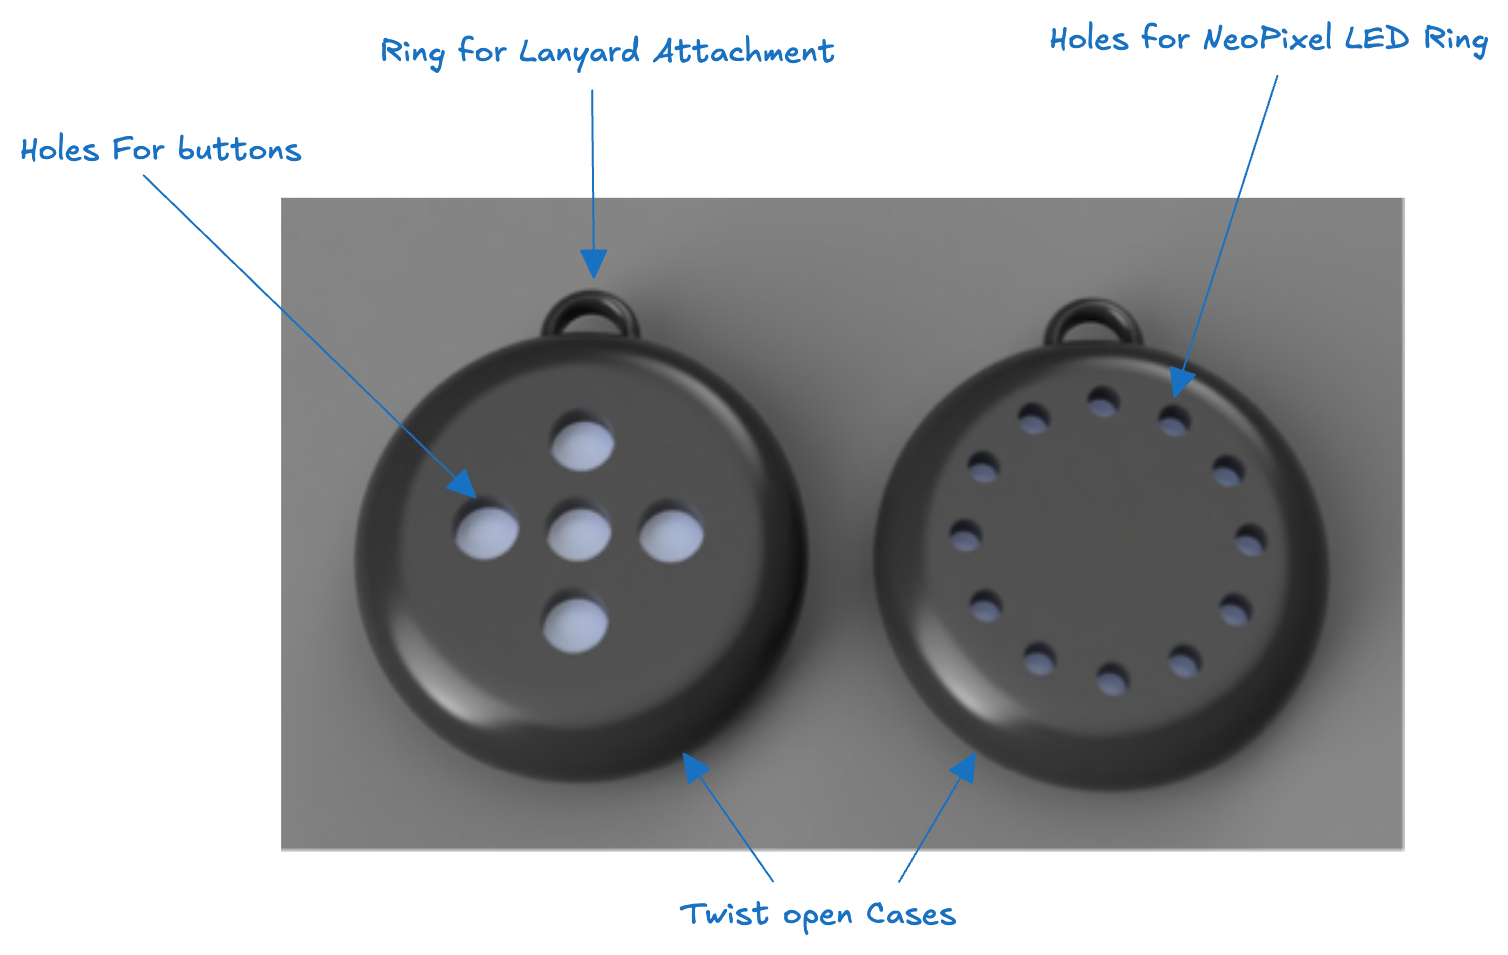
\includegraphics[width=0.55\textwidth]{labeled_render.png}
    \caption{Skip's device (left) and sweeper's device (right). Both devices are 65mm in diameter and 25mm thick.}
    \label{fig:device}
\end{figure}

\begin{figure}[ht!]
    \centering
    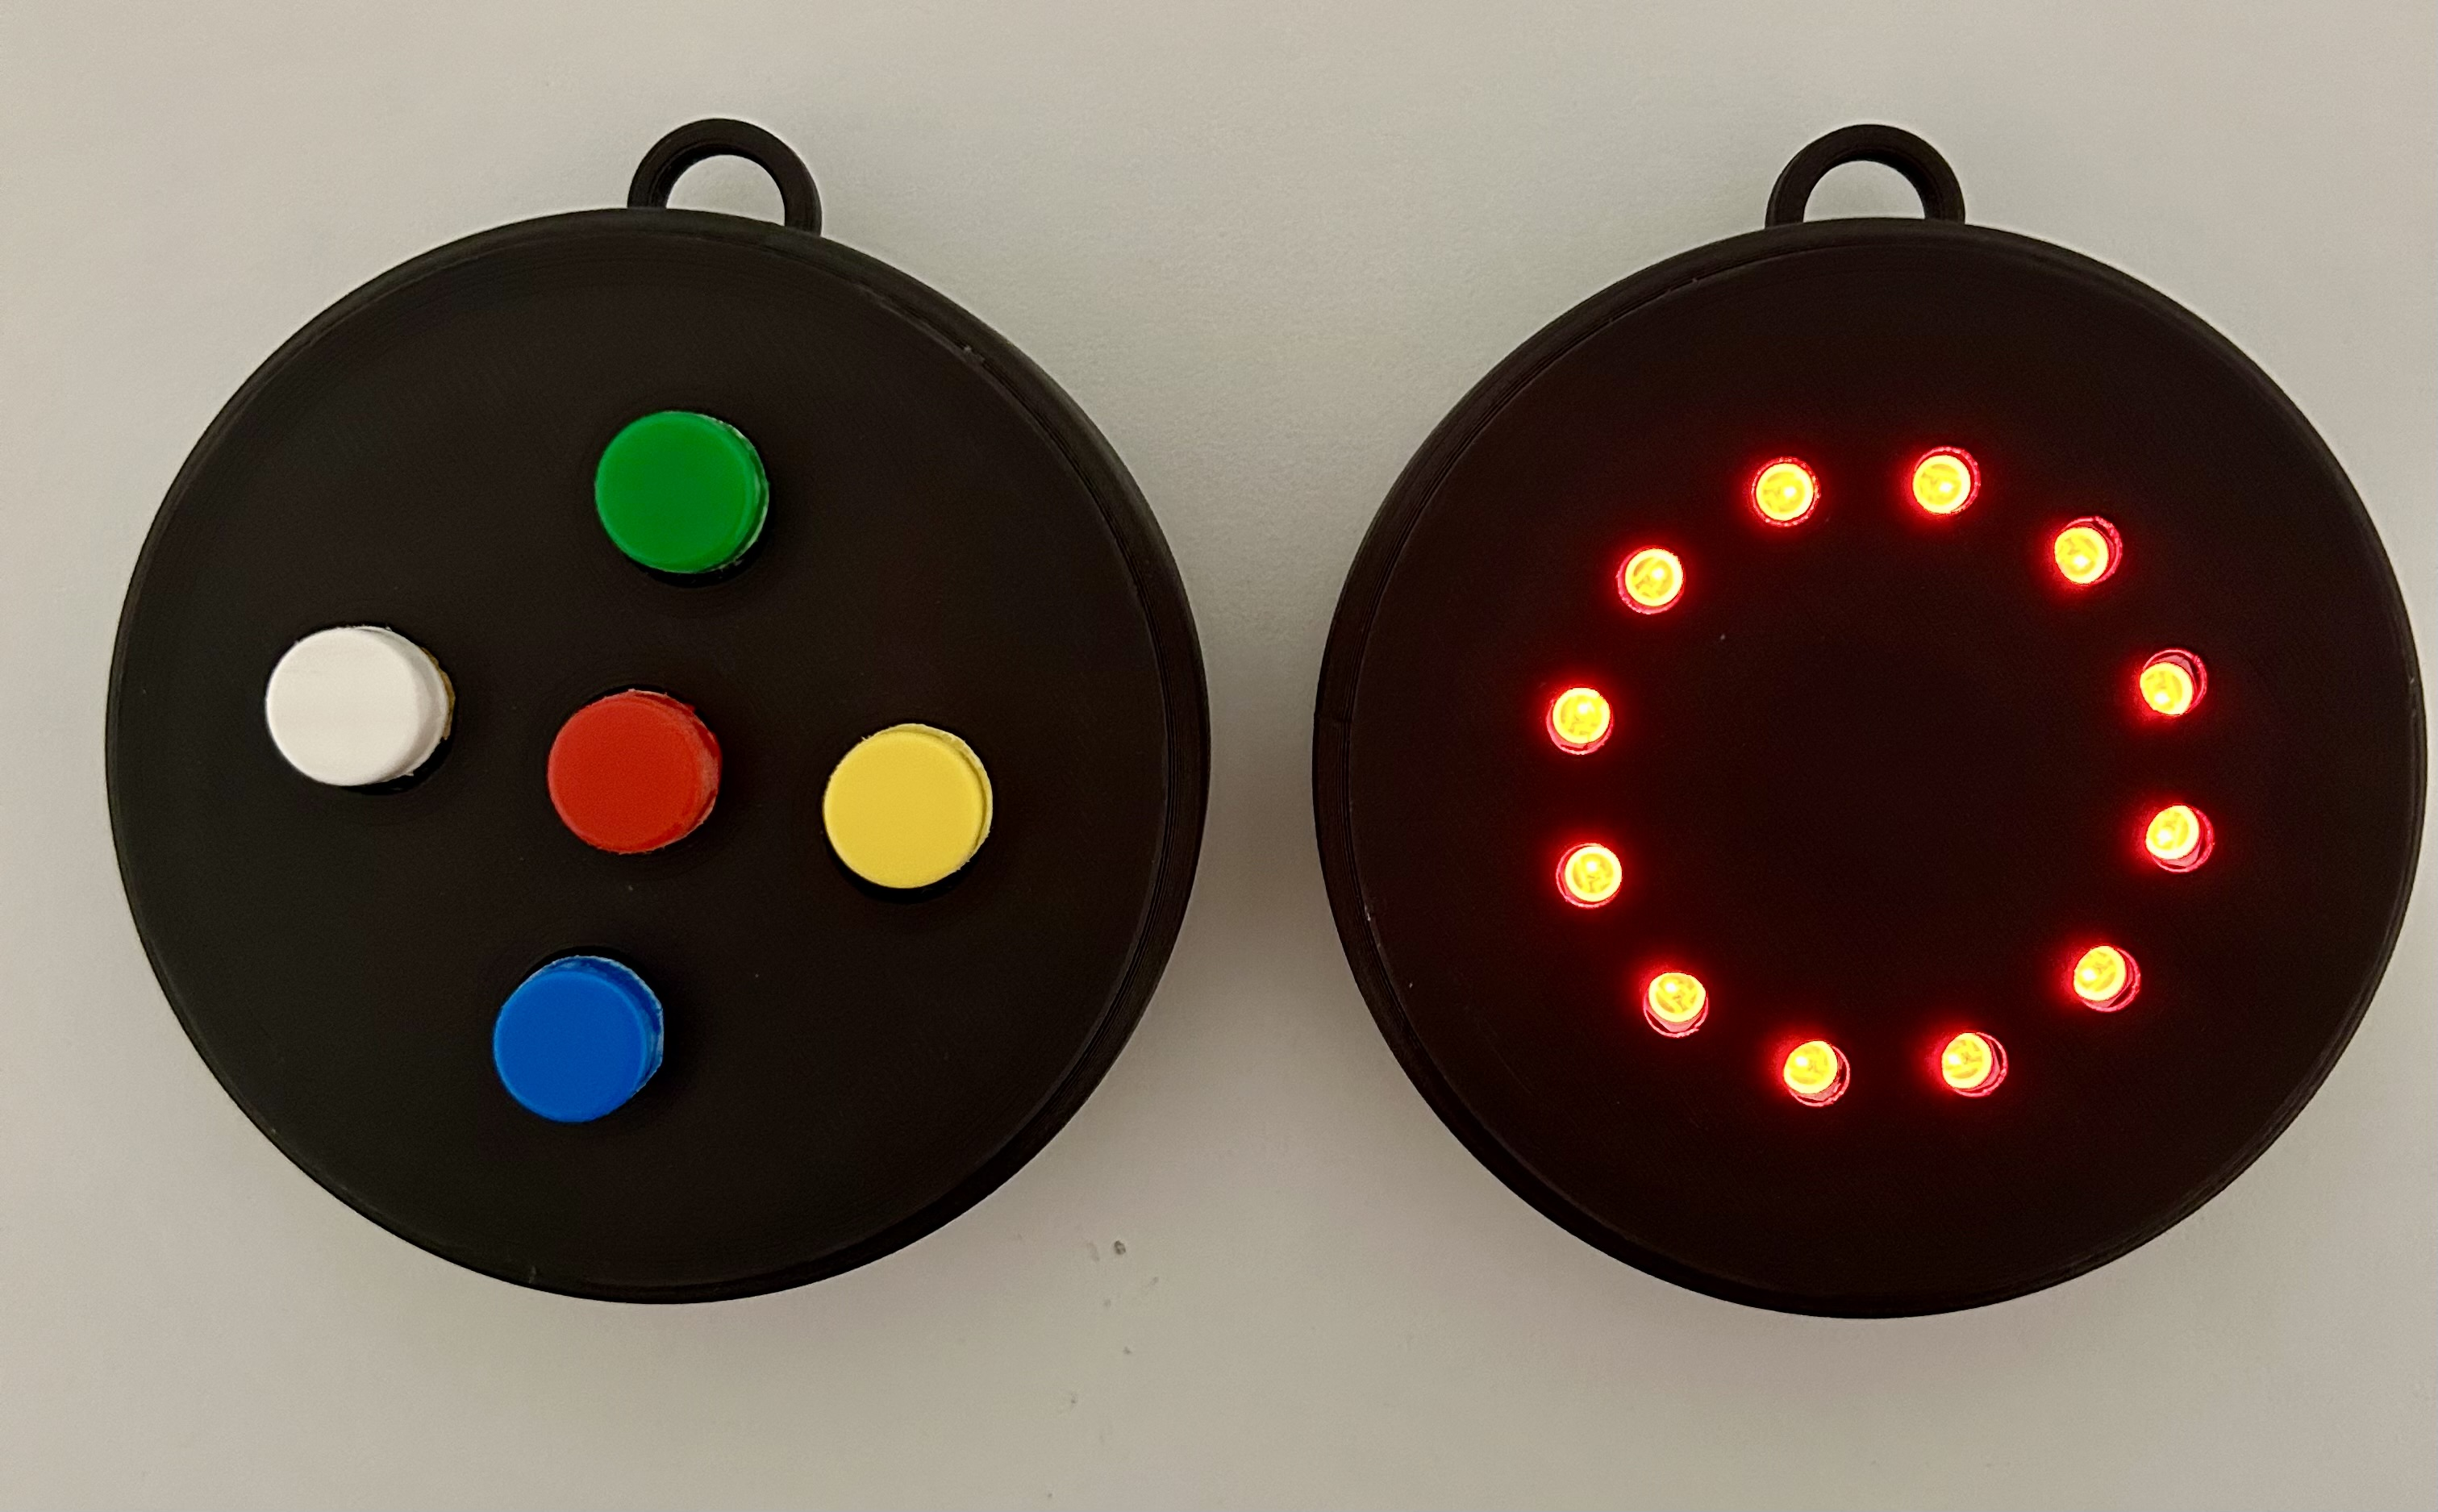
\includegraphics[width=0.50\textwidth]{device_assembled.jpeg}
    \caption{Skip's device (left) and sweeper's device (right) fully assembled}
    \label{fig:built_devices}
\end{figure}
% TODO: include drawings

\subsection{Background of the Invention}
Curling is a sport that relies heavily on verbal communication between players, particularly between the skip and the sweepers. These verbal cues are essential for guiding the sweepers on when to sweep, how hard to sweep, and how to adjust based on the rock's trajectory. Deaf curlers face a significant disadvantage, as they are unable to hear these commands and must constantly look toward the skip for direction, reducing their ability to focus on the stone.

The idea for this invention arose from recognizing this accessibility gap. The aim is to create a solution that levels the playing field, allowing deaf athletes to fully engage in the sport without communication barriers. By replacing verbal communication with a visual signaling system, the invention enables real-time, hands-free communication on the ice in a way that is both functional and discreet.

The proposed system is a wireless communication device that allows the skip to send distinct visual signals to the sweepers' devices. This helps remove the need to look back at the skip for instructions, allowing sweepers to maintain their focus on the stone and the game.



\subsection{Summary of the Disclosure}
According to the World Curling Federation (WCF) rules\footnote{\url{https://worldcurling.org/wp-content/uploads/2024/08/Rules-2024.pdf}}, section R11(c) prohibits the use of most electronic devices on the ice, except in cases of medical necessity. The relevant section reads:

\textbf{R11 (c)}: \textit{Teams must not use electronic communication equipment, or any device to modify the voice, during a game. With the exception of stopwatches that are limited to providing 'time' data only, the use of electronic devices during the games, which provide information to players on the athletes' field of play, are forbidden. A whistle or another signalling instrument can be used in case of medical reason and after consultation and written approval from World Curling.}

In this context, the proposed device qualifies as a signaling instrument used for medical reasons. It does not provide any extra game-related information as compared to shouting the commands. The device is solely intended to enable equitable participation for deaf athletes, in alignment with the spirit of the WCF's medical exception clause.

Furthermore, the attachment of the device to the broom is also allowed as currently timers are allowed and are often attached to the broom. Although according to C3 (d), the broom must be prequalified by the WCF and shall not be exchanged during the game. Our invention does not require sweepers to swap brooms as each sweeper would have their own device and is therefore compliant with this rule.

\textbf{C3 (d)}: \textit{Each player must declare an approved sweeping device at the start of a game, and only that player can use that device for sweeping during the game.}


\subsection{Brief Description of the Drawings}

The drawings depict two similar shaped devices, one for the skip, with it's 5 buttons, and one for the sweepers, with its LED ring. Both devices have a similar form factor to a stopwatch, which is a common tool in curling. The devices both have a hook to attach to a lanyard, or alternatively, a belt clip. The sweeper's device is intended to be attached to the broom, ensuring it is always in the line of sight of the sweepers. However, this is not a requirement and the device can be used in any position that is comfortable for the user.

The 5 distinct buttons on the skip's device are designed to be easily identifiable by location and color. Each button corresponds to a specific command, which is transmitted wirelessly to the sweeper's device.

The LED ring on the sweeper's device is designed to be easily visible in bright lighting conditions, ensuring that the sweepers can receive commands without needing to look back at the skip. The LED ring displays one of five distinct visual patterns, each clearly mapped to one of the commands. These patterns are designed to be easily recognizable during gameplay, even in bright lighting conditions. The devices are both 65mm in diameter and 25mm thick.

\subsection{Detailed Description of the Invention}

The system consists of two primary components:
\begin{itemize}
    \item A remote control operated by the skip, worn on a lanyard around the neck
    \item A receiver unit attached to the sweepers' broom, shaped similarly to a stopwatch. Intended to be attached on the broom ensuring it is always in the line of sight of the sweepers.
\end{itemize}

Both devices are powered by rechargeable batteries and utilize the ESP32 microcontroller for control. Communication between the devices is handled using ESP-NOW, a low-power, low-latency wireless protocol ideal for short-range communication.

The skip's remote control features five buttons, each corresponding to a unique command. These commands are transmitted wirelessly to the sweepers' device.

On the receiver, an LED ring displays one of five distinct visual patterns, each clearly mapped to one of the commands. These patterns are designed to be easily recognizable during gameplay, even in bright lighting conditions. The device is also lightweight, ensuring it does not interfere with sweeping technique or performance.

The unit's form factor is intentionally similar to a stopwatch, a familiar and widely accepted tool in curling, minimizing visual distraction for players and spectators. Its appearance and function are both unobtrusive and in line with standard curling equipment, ensuring it does not disrupt the aesthetics or flow of the game.

The wireless communication is designed to be power efficient. Commands are only sent in periodic intervals, and when the skip is not sending commands for a certain period of time, both devices enter a lower-power state. This ensures that the devices can last through an entire game without needing to be recharged. Both devices have removable batteries or they can be charged using a USB. The devices twist apart to allow for easy battery replacement.


Lastly, \autoref{fig:commands} depict the five commands and their corresponding LED patterns. The stop pattern can be seen in the fully assembled device in \autoref{fig:built_devices}.  

\begin{figure}[ht!]
    \centering
    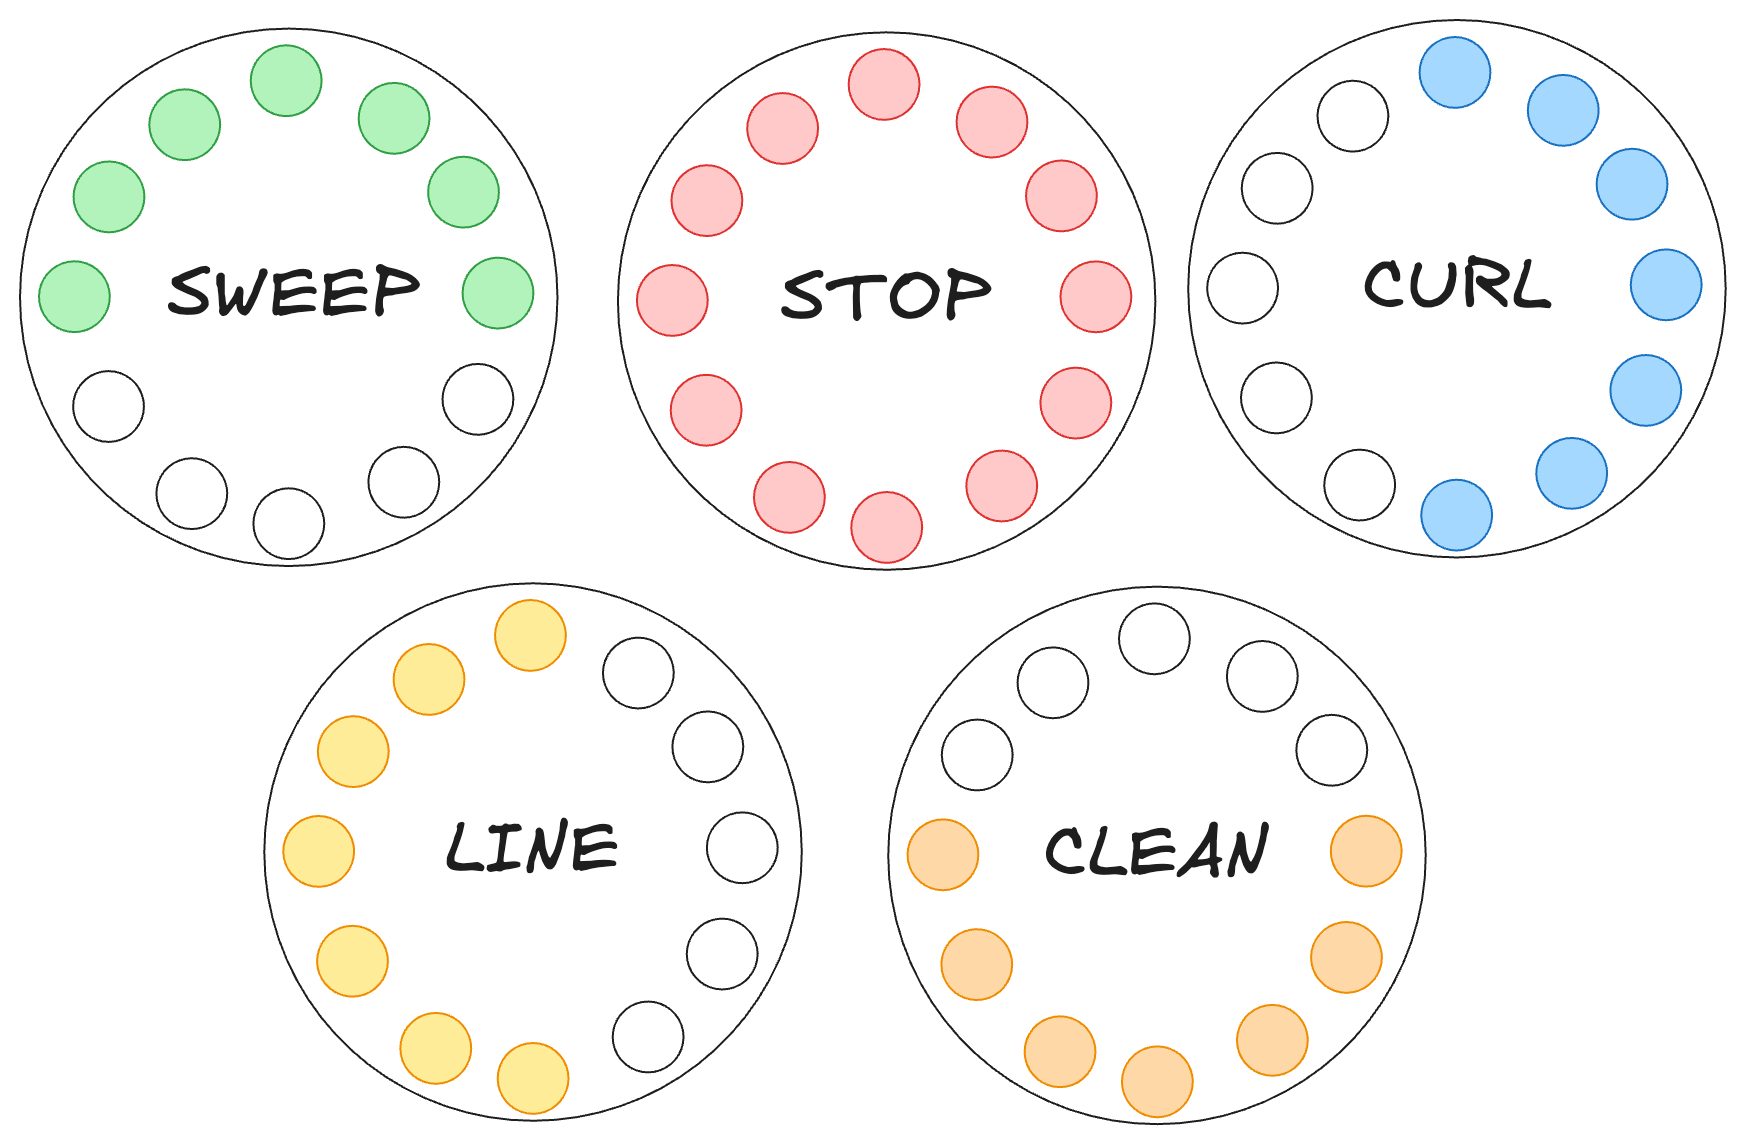
\includegraphics[width=0.5\textwidth]{commands.png}
    \caption{Commands and their corresponding LED patterns}
    \label{fig:commands}
\end{figure}


\subsection{Claims}
Only one claim is made in this application:

A visual communication system that allows a curling skip to send distinct non-verbal signals to sweepers through wireless transmission to broom-mounted visual display devices.



% --------------------------------------------------------------------------------
% END BODY
% --------------------------------------------------------------------------------

\end{document}
